O programa \emph{Matlab\tiny\textregistered} dispõe de um ambiente de simulações ( Simulink ) que possibilita através de montagem de diagramas de blocos que contenham funções, elementos de circuitos, modelagens, etc. fazer simulações matemáticas desses sistemas e auxiliar o projetista encontrar a melhor situação  do projeto em execução. 

No nosso caso será usado para promover o melhor resultado de ajustes para os parâmetros de ganho do sistema \emph{PID}.\\

As informações e instruções de uso deste aplicativo estão sendo tiradas do livro da própria \emph{Matworks \tiny\textcopyright}  \cite{userguide}.
Para o ilustrar a utilização pretendida do aplicativo Simulink, abaixo temos uma figura de um esquema de blocos para um sistema utilizando \emph{PDI}:

\begin{figure}[H]
		\centering
		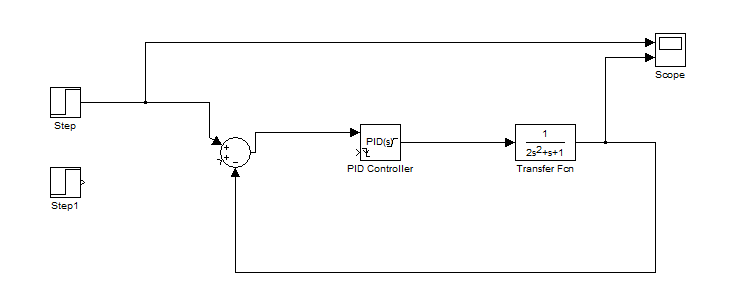
\includegraphics[width=0.8\linewidth]{./ima/DiaBlocos01.png}
		%\caption{}
		\label{fig:fluxo1}
		\caption{Diagrama De Blocos - Simulink}
	\end{figure}
	
Ensaiando esse circuito no aplicativo, temos como resultados os gráficos abaixo, sendo que no primeiro temos um pulso de 5V em 20s  e vemos a resposta para os parâmetros do \emph{PDI} sem ajuste correto que pode-se ver apresentar oscilações antes de equilibrar o sinal:

\begin{figure}[H]
		\centering
		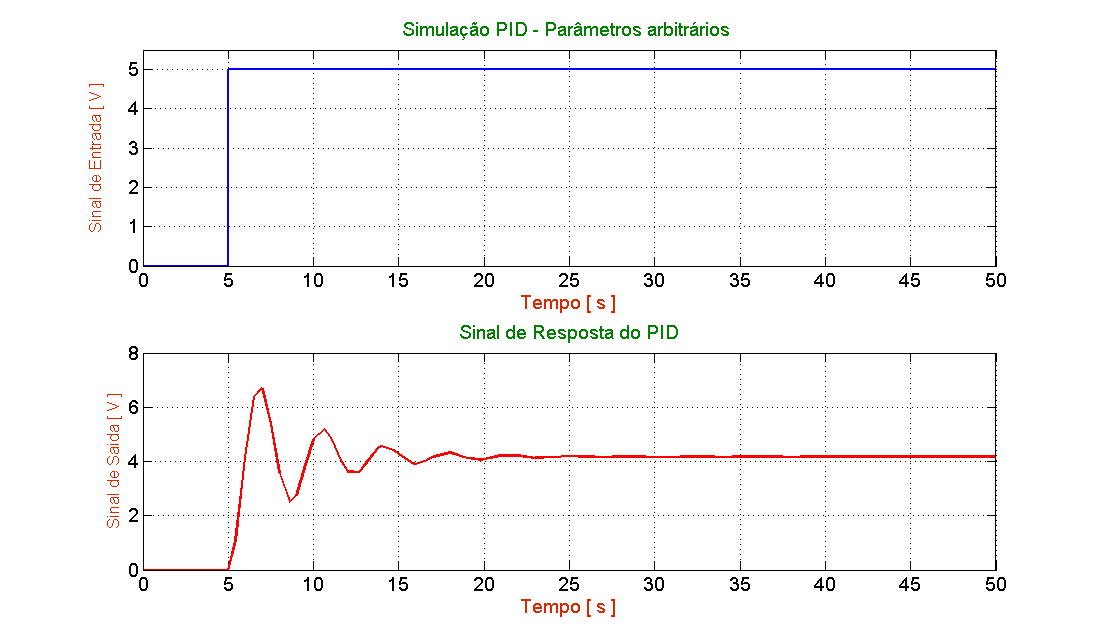
\includegraphics[width=0.9\linewidth]{./ima/GrafRegulado2.png}
		%\caption{}
		\label{fig:fluxo1}
		\caption{Gráfico - Ensaio 01 sem parâmetros}
	\end{figure}
	
Neste próximo gráfico, temos o mesmo circuito acima sendo ensaido com os parâmetros sugeridos pelo aplicativo Simulink, onde podemos ver uma resposta melhor para o sistema para as mesmas condições do gráfico acima:

\begin{figure}[H]
		\centering
		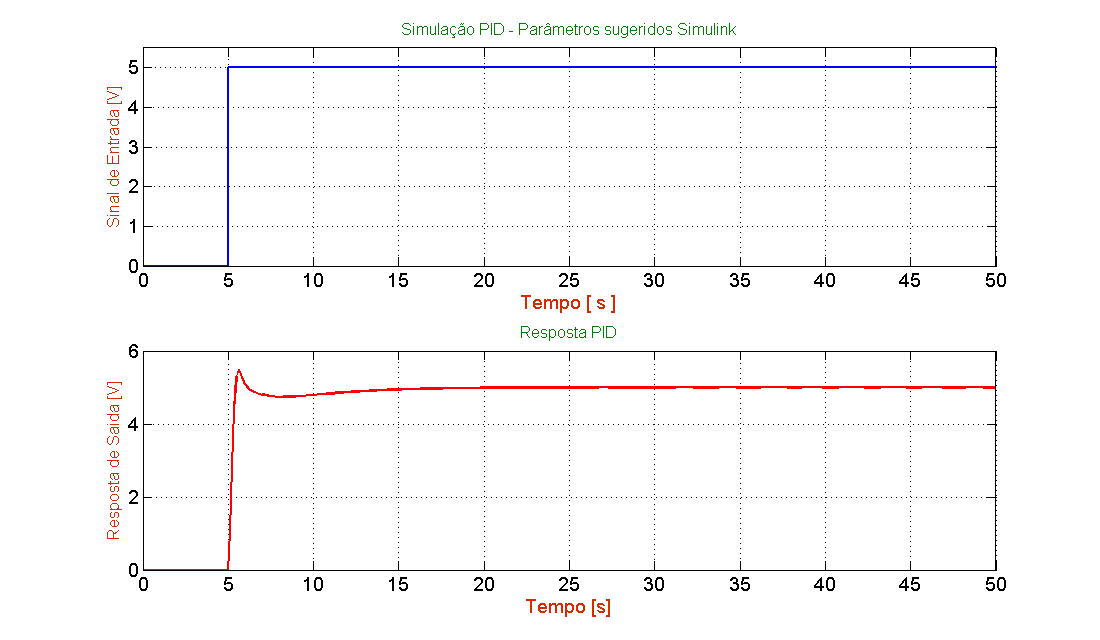
\includegraphics[width=0.9\linewidth]{./ima/GrafRegulado1.png}
		%\caption{}
		\label{fig:fluxo1}
		\caption{Gráfico - Ensaio 02 com parâmetros corrigidos}
	\end{figure}
	
Assim com auxilio destes recursos, poderemos obter um sistema \emph{PDI} com bons parâmetros de resposta para podermos passar para simulações de circuitos e finalmente montagem do protótipo tentando corrigir possíveis desvios. 

Isso faz que se ganhe tempo e possa obter maiores informações antes mesmo de se necessitar montar um circuito genérico para testes.

